\textbf{{1. 在双链表L尾部插入值为key的结点}}

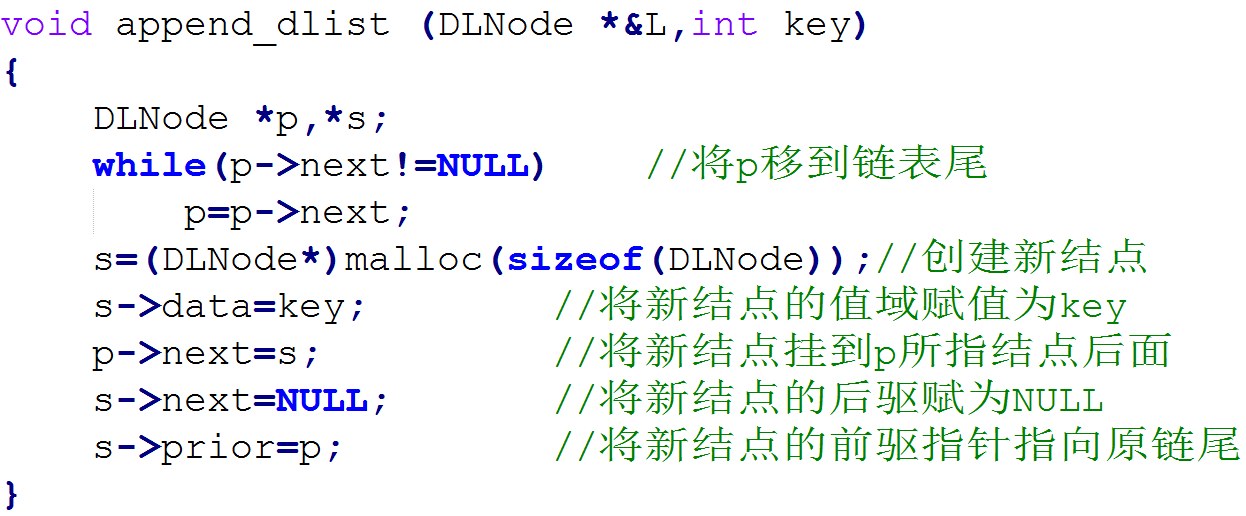
\includegraphics[width=3.33333in,height=1.38542in]{png-jpeg-pics/03268EAA15CD33F53F293BD78E598542.png}

\textbf{{2. 查找双链表L结点值为key的结点,找到返回其地址,否则返回NULL}}

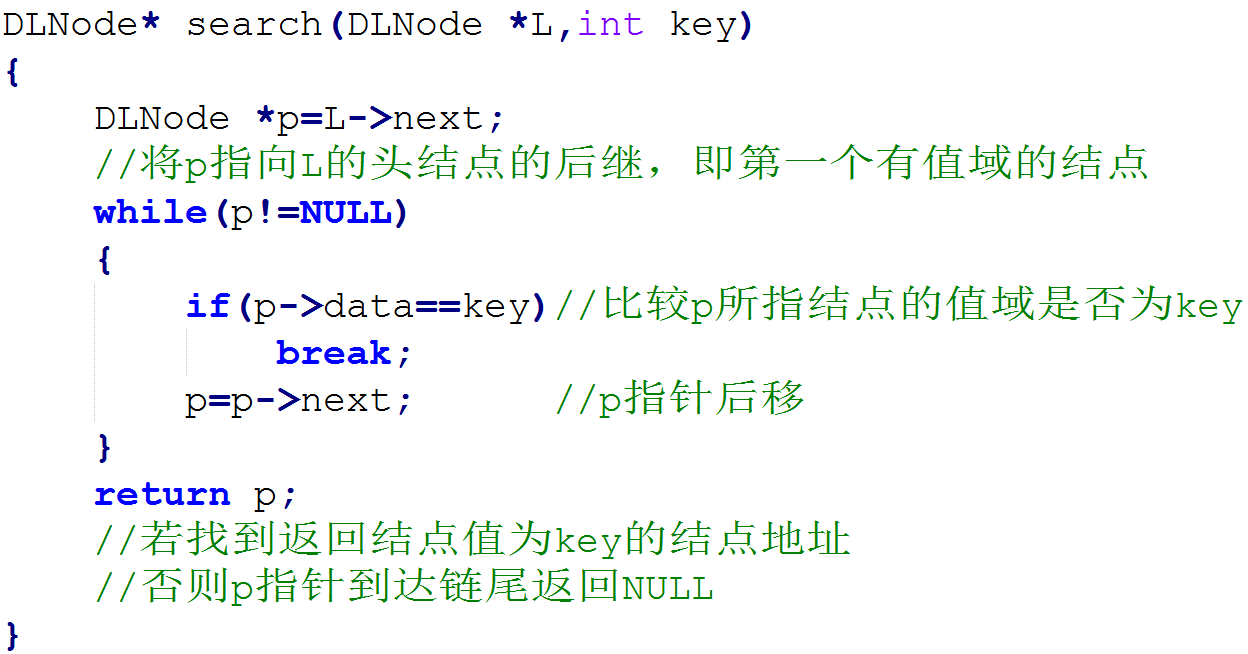
\includegraphics[width=3.33333in,height=1.75000in]{png-jpeg-pics/01B96410D375D9482DBD49E4733D199A.png}

\textbf{{3.
在双链表中p所指结点之后插入结点s,其中p结点不是最后一个结点}}

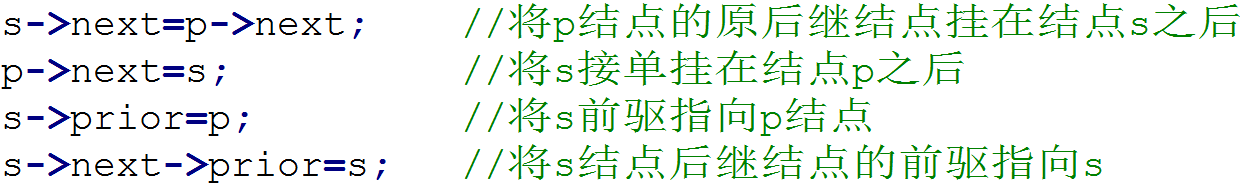
\includegraphics[width=3.43750in,height=0.51042in]{png-jpeg-pics/1E0D67141EAF5766A73E880D92654FFF.png}

\textbf{{注意:第一行和第二行一定要记住,先写这两句,就不会错。}}

\textbf{{4. 在双链表中删除p结点的后继结点}}

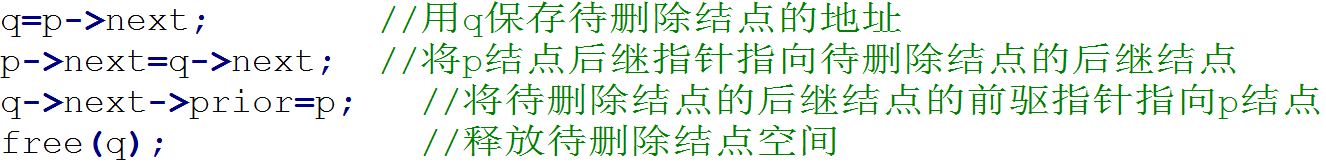
\includegraphics[width=3.43750in,height=0.42708in]{png-jpeg-pics/5F88607817AE7DD214FE9DF244A7CE02.png}
